\begin{figure}%[!htbp]
\begin{center}

\begin{subfigure}[b]{0.5\columnwidth}
  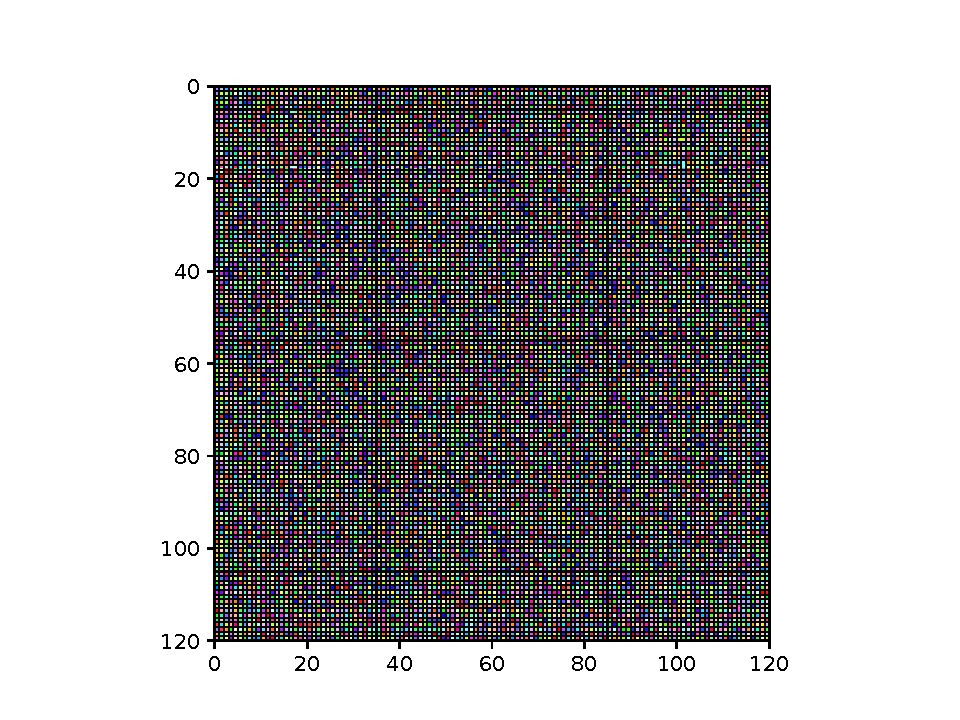
\includegraphics[width=\columnwidth,trim={2.5cm 0.5cm 2.5cm 1cm},clip]{img/ChannelMap_1007_update0}
  \caption{Cell gen. 0}
  \label{fig:ChannelMap_1007_update0}
\end{subfigure}%
\begin{subfigure}[b]{0.5\columnwidth}
  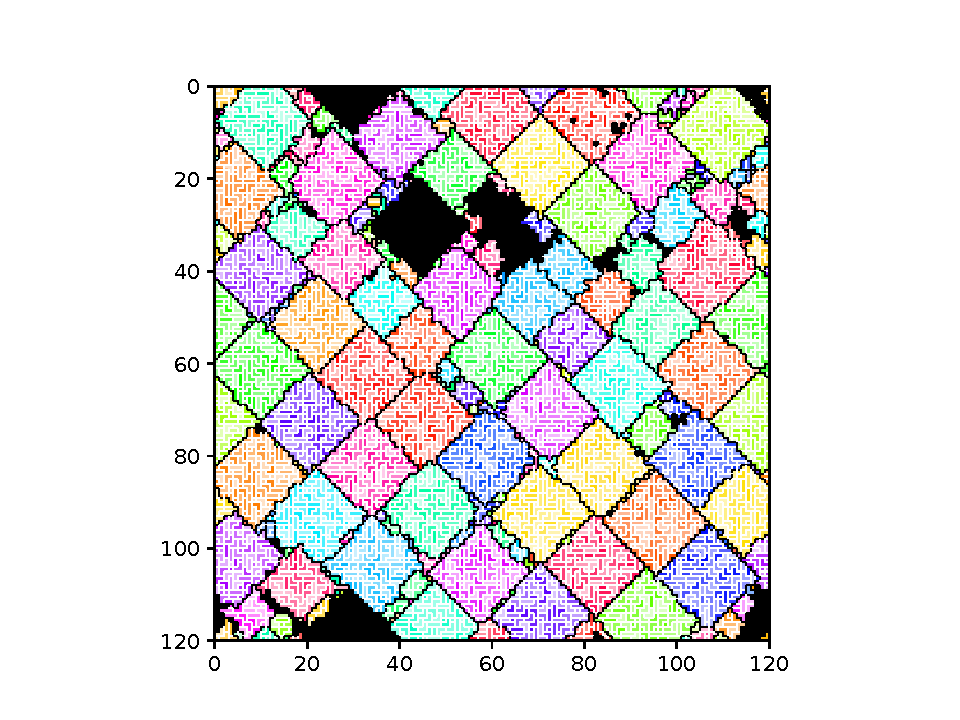
\includegraphics[width=\columnwidth,trim={2.5cm 0.5cm 2.5cm 1cm},clip]{img/ChannelMap_1007_update2000000}
  \caption{Cell gen. 4974}
  \label{fig:ChannelMap_1007_update2000000}
\end{subfigure}

\caption{
Progression of of same-channel level-one and level-two signaling networks states in an evolutionary run where level-two resource sharing evolved.
Level-one channels are coded by color saturation and level-two channels are coded by color hue.
A single cell-like organism occupies each grid tile except for black tiles, which are empty.
}
\label{fig:grid_progression}
\end{center}
\end{figure}
